
\section{mpolishing.rb - Polish general graph\label{sect:mpolishing}}

Data polishing algorithm can be applied to general graph data to remove noise, and generate "polished graph" to increase distinction of graph.  
In order to illustrate the effect of polishing, Figure \ref{fig:polish0} and Figure \ref{fig:polish1} shows the graphs before and after polishing respectively.   
In the original graph, the dense structure is polished to enhance the density, while the sparse structure is thinned out. 
As a result, many medium-sized maximal cliques (other complete subgraph that does not exists exclusively in complete subgraph) are generated. 


\begin{figure}[htbp]
\begin{center}
\begin{tabular}{cc}

\begin{minipage}{0.3\hsize}
\begin{center}
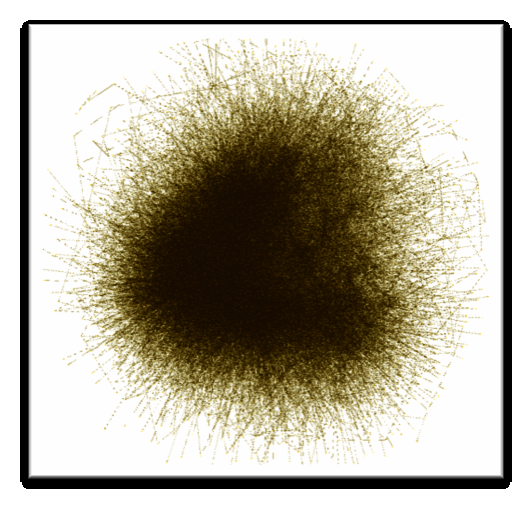
\includegraphics[scale=0.5]{./polish0.eps}
\caption{Graph before polishing\label{fig:polish0}}
\end{center}
\end{minipage}

\begin{minipage}{0.3\hsize}
\begin{center}
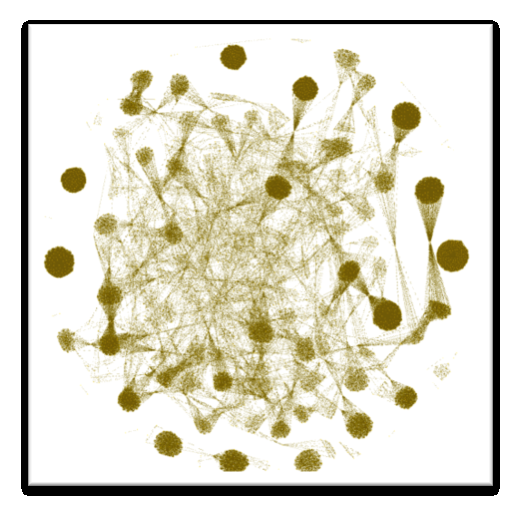
\includegraphics[scale=0.5]{./polish1.eps}
\caption{Graph after polishing\label{fig:polish1}}
\end{center}
\end{minipage}

\end{tabular} 
\end{center}
\end{figure} 

The polishing algorithm is shown in Algorithm \ref{algo:polish}. 
The algorithm shown below  is not the most efficient but the mechanics shows how it works. 
Please refer to \cite{Uno2014} for  detailed reference on the algorithm which was implemented in the command.  
Polishing is based on a simple methodology by  connecting all pairs of nodes (vertices) if the degree of similarity is more than or equal to threshold specified by user, otherwise, a new graph will be created from rules that were not connected. 


\begin{algorithm}
\caption{Graph polishing algorithm \label{algo:polish}}
\begin{small}
\begin{algorithmic}[1]
\Function{Polishing}{$G=(V,E),\sigma$}
	\State $V:Vertex set, E:Edge set, \sigma: Lower limit of similarity$
	\State $E'=\phi$; $V'=\phi$ \Comment Initialization of edge set and vertex set after polishing
	\ForAll{$u\in V$}
		\ForAll{$v\in V$} \Comment \# Search for all vertex pair $u,v$
			\If{$sim(u,v)\ge\sigma$} \Comment If the vertices pair $u,v$ are similar, add a new edge, otherwise, do not add 
				\State $E'=E'\cup (u,v)$
				\State $V'=V'\cup u$
				\State $V'=V'\cup v$
			\EndIf
		\EndFor
	\EndFor
	\State {\bf return}{$(V',E')$}
\EndFunction
\end{algorithmic}
\end{small}
\end{algorithm}

The same polishing procedure is repeatedly applied to newly constructed graph until there are no more changes to the graph structure, or when the number of iterations reaches the maximum value specified by user. The final graph obtained is the polished graph.  

The definition of similarity between two nodes (Refer to line 6 of Algorithm \ref{algo:polish}:$sim(u,v)$) is shown. Basically, let's consider "Friends who have a lot of common friends".   
Figure \ref{fig:sim} shows the structure where the nodes in the middle are  connected to nodes $u,v$.
 Even though $u$ and $v$ are not directly connected, among the 5 connected nodes, nodes 3,4 have 2 common nodes connected.   
 This information is used to define degree of similarity. 
 
\begin{figure}[htbp]
\begin{center}

\begin{minipage}{0.3\hsize}
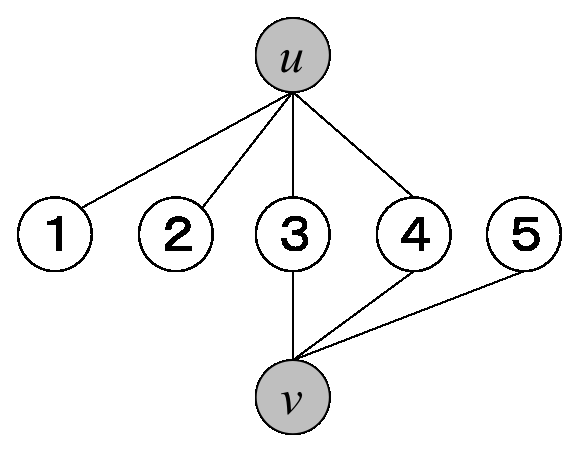
\includegraphics[scale=0.5]{./sim.eps}
\caption{Connection relationship of vertex $u,v$\label{fig:sim}}
\end{minipage}
\end{center}
\end{figure}

There are 6 types of similarity measures which can be applied in this command as shown in \ref{tbl:simdef}. The desired similarity measure can be defined at the \verb|sim=| parameter,  and the lower limit of degree of similarity can be specified at \verb|th=| parameter. 


\begin{table}[htbp]
\begin{center}
\caption{Similarity definition of graph $G=(V,E)$ with nodes $u,v$\label{tbl:simdef}}
%{\small
\begin{tabular}{cllcc}
\hline
\# & Degree of Similarity&Equation&sim= parameter&Range \\
\hline
1&resemblance    & $\frac{|N(u) \cap N(v)|}{|N(u) \cup N(v)|}$ & R & 0.0〜1.0\\
2&normalized PMI & $\log{\frac{P(u,v)}{P(u)P(v)}}/(-\log{P(u,v)})$ & P  & -1.0〜1.0\\
 &               & $=\frac{|V||N(u) \cap N(v)|}{|N(u)||N(v)|}/(-\log{\frac{|N(u) \cap N(v)|}{|V|}})$ & \\
3&intersection   & $|N(u) \cap N(v)|$ & T & 0〜\\
4&cosine         & $\frac{|N(u) \cap N(v)|}{\sqrt{|N(u)|}\sqrt{|N(v)|}}$ & C  & 0.0〜1.0\\
5&max-confidence & $\frac{|N(u) \cap N(v)|}{\max{(|N(u)|,|N(v)|)}}$ & S  & 0.0〜1.0\\
6&min-confidence & $\frac{|N(u) \cap N(v)|}{\min{(|N(u)|,|N(v)|)}}$ & s  & 0.0〜1.0\\
\hline
\end{tabular} 
\\
{\scriptsize
$N(u)$ denotes the set of nodes adjacent to node $u$.
$P(u)$ represents the probability that the edge will reach node $u$ where $P(u)=N(u)/|V|$.
}
\end{center}
\end{table}

\subsection{Examples}
Input data of general graph for this command is shown in Table \ref{tbl:input}, edge data and node pair is expressed in CSV format. 
The graph is processed as undirected graph, with multiple islands. 
Single node which does not have an edge is not subjected to polishing (no friend), and the node data is not used as input. Data shown in Table \ref{tbl:input} is visualised as graph format in Figure \ref{fig:inputg}. 
Example of data polishing using the sample data is shown below. 

\vspace{1em}

\begin{table}[htbp]
\begin{center}
\caption{Input Data (Edge data)\label{tbl:input}}
\begin{tabular}{cc}
\hline
node1&node2 \\
\hline
a&b\\
a&c\\
a&e\\
b&c\\
b&e\\
b&g\\
c&d\\
c&g\\
d&e\\
e&f\\
\hline
\end{tabular} 
\end{center}
\end{table} 

For simplicity, similarity is defined as intersection with a lower limit of 2. 
In other words, when the adjacent nodes has 2 or more common nodes, extend the edge, and  vice versa. 
For example, Figure \ref{fig:ad}, Figure \ref{fig:inputg} is a subgraph extracted of which are connected with nodes $a,b$.  
Having the 2 nodes $e,c$ in common, the edge of node $a,b$  is extended in the polished graph. 
 While the common node for $e,g$(Figure \ref{fig:eg}) is only $b$, the edge is not extended in the polished graph.  

\begin{figure}[htbp]
\begin{center}
\begin{tabular}{ccc}

\begin{minipage}{0.3\hsize}
\begin{center}
\includegraphics[scale=0.5]{./inputg.eps}
\caption{Visualization of graph data in Table \ref{tbl:input}\label{fig:inputg}}
\end{center}
\end{minipage}

\begin{minipage}{0.2\hsize}
\begin{center}
\includegraphics[scale=0.5]{./ad.eps}
\caption{Relationship between node $a$ and node $d$\label{fig:ad}}
\end{center}
\end{minipage}

\begin{minipage}{0.2\hsize}
\begin{center}
\includegraphics[scale=0.5]{./eg.eps}
\caption{Relationship between node $e$ and node$g$\label{fig:eg}}
\end{center}
\end{minipage}

\end{tabular}
\end{center}
\end{figure}

Figure \ref{fig:ab2} shows a subgraph related to node $a,b$. The difference from the past 2 examples is that nodes $a,b$ are directly connected. In this case, there are two consideration. 
First, in Figure \ref{fig:ab1}, without considering direct relationship, only take into account common relationships with friends. 
The other method assumes nodes $a,b$ have common friends, fictitious node $a',b'$ is added, and it is assumed that both $a,b$ are connected as shown in Figure \ref{fig:ab3}. 
Therefore, if there is a direct connection, there will only be two people as common friends. 


\begin{figure}[htbp]
\begin{center}
\begin{tabular}{ccc}

\begin{minipage}{0.3\hsize}
\begin{center}
\includegraphics[scale=0.5]{./ab2.eps}
\caption{Relationship between node $a$ and node $b$\label{fig:ab2}}
\end{center}
\end{minipage}

\begin{minipage}{0.3\hsize}
\begin{center}
\includegraphics[scale=0.5]{./ab1.eps}
\caption{Example without  direct connection\label{fig:ab1}}
\end{center}
\end{minipage}

\begin{minipage}{0.3\hsize}
\begin{center}
\includegraphics[scale=0.5]{./ab3.eps}
\caption{Example with direct connection\label{fig:ab3}}
\end{center}
\end{minipage}

\end{tabular}
\end{center}
\end{figure}


When updating new connection relationship for all nodes pairs as described above, the polished graph excluding direct relationship is shown in Figure \ref{fig:polished0}, and the polished graph with direct relationship is shown in Figure \ref{fig:polished2}. When the newly graphs are repeatedly polished and the graph structure did not change (converge) for 3 times, Figure \ref{fig:polished1} and Figure\ref{fig:polished3} are obtained. 
When direct connection is not considered, all relationship connections are removed. On the other hand, if direct connect is considered, the six nodes $a,b,c,d,e,g$ are connected to each other and maximal cliques are created. 
However, node $f$ is still connected with $e$, which also forms maximal cliques $e,f$.  Finally, when data polishing is repeated applied, the graph structure will gradually be stabilized. However, in some cases, the structure does not converge. 


\begin{figure}[htbp]
\begin{center}
\begin{tabular}{cccc}

\begin{minipage}{0.25\hsize}
\begin{center}
\includegraphics[scale=0.5]{./polished0.eps}
\caption{Graph polished once without direct connection\label{fig:polished0}}
\end{center}
\end{minipage}

\begin{minipage}{0.25\hsize}
\begin{center}
\includegraphics[scale=0.5]{./polished1.eps}
\caption{Graph polished 3 times without direct connection\label{fig:polished1}}
\end{center}
\end{minipage}

\begin{minipage}{0.25\hsize}
\begin{center}
\includegraphics[scale=0.5]{./polished2.eps}
\caption{Graph polished once with direct connection\label{fig:polished2}}
\end{center}
\end{minipage}

\begin{minipage}{0.25\hsize}
\begin{center}
\includegraphics[scale=0.5]{./polished3.eps}
\caption{Graph polished 3 times with direct connection\label{fig:polished3}}
\end{center}
\end{minipage}

\end{tabular}
\end{center}
\end{figure}


Similarity in simple terms, can be defined as the  number of edges in common for data polishing. However, as the size of the graph increases, there are more cases where the edges cannot be polished. As the number of adjacent nodes increases, the number of nodes become huge, even when edges are extended for nodes pairs sharing common nodes, the relationship is relatively weak.  

Therefore, by applying resemblance, the degree of similarity can be used to evaluate relative common similarity measure. When resemblance is used as similarity measure,  graphs that are polished until convergence at lower limit at 0.4 and 0.5 is shown in Figure \ref{fig:resemblance04} and \ref{fig:resemblance05}.

Figure \ref{fig:pmi02} is a result of applying normalized PMI as degree of similarity, with a lower limit of 0.2.


\begin{figure}[htbp]
\begin{center}
\begin{tabular}{ccc}

\begin{minipage}{0.3\hsize}
\begin{center}
\includegraphics[scale=0.5]{./resemblance04.eps}
\caption{Polished graph with resemblance=0.4\label{fig:resemblance04}}
\end{center}
\end{minipage}

\begin{minipage}{0.3\hsize}
\begin{center}
\includegraphics[scale=0.5]{./resemblance05.eps}
\caption{Polished graph with resemblance=0.5\label{fig:resemblance05}}
\end{center}
\end{minipage}

\begin{minipage}{0.3\hsize}
\begin{center}
\includegraphics[scale=0.5]{./pmi02.eps}
\caption{Polished graph with normalized PIM=0.2\label{fig:pmi02}}
\end{center}
\end{minipage}

\end{tabular}
\end{center}
\end{figure}

Other than the polished graph, various operation statistics can be returned in the output as shown in Table \ref{tbl:stat} (File specified at \verb|log=|).

\begin{table}[htbp]
\begin{center}
\caption{Statistics to be displayed in log file\label{tbl:stat}}
%{\small
\begin{tabular}{ll}
\hline
Key & Description \\
\hline
iter & Iterations for data polishing  \\
time & Execution time\\
nSize0 & Number of graph nodes before polishing \\
eSize0 & Number of graph edges before polishing \\
dens0  & Density of edges before polishing  \\
nSize\# & Number of nodes after \# polishing iterations \\
eSize\# & Number of edges after \# polishing iterations \\
dens\#  & Density of edges after \# polishing iterations \\

\hline
\end{tabular} 
\end{center}
\end{table}


The characteristics of data polishing is summarized below. 
\begin{itemize}
\item Extend edges according to information on common adjacent nodes. 
\item Select from 6 types of similarity measures, the results vary according to the type of similarity measure. 
\item The graph structure is stabilised by iterating data polishing cycles (converges at most times). 
\item Number of maximal cliques is reduced drastically when compared to the original graph. 
\item Maximal cliques are formed when the lower limit of degree of similarity decreases. 
\end{itemize}


\subsection{Format}
\begin{verbatim}
mpolishing.rb i= f= o= [sim=R|P|C|s|S|T] th= [sup=] [-int] [-indirect] [iter=] [log=] [T=] [--help]

  Specification of file 
  i=     : Edge data file
  f=     : Field name of 2 nodes in edge data (cannot be used when -int is specified)
  o=     : Edge data file after data polishing
  sim=   : Definition of degree of similarity as benchmark for edge extension  
              R: resemblance
             P: normalized PMI
             C: cosine
             S: max-confidence
             s: min-confidence
             T: intersection
  th=    : Lower limit of degree of similarity (specified by sim=) as benchmark for edge extension 
  sup=   : Add the condition intersection>=sup for the calculation of similarity. Default is set as sup=0 if not defined. When sim=T is defined, this parameter will not be meaningful. 
  -int   : Treat item as integer for processing. 
  -indirect: Exclude direct relationship  for adjacent nodes when calculating degree of similarity. 
  iter=  : Maximum number of iterations for data polishing (default=30)
  log=   : Output file name of parameter settings and convergence information in CSV key-value format. 

Others
  T= : Working directory (default:/tmp)
  O=     : Directory name to save the data from polishing process in debug mode 
  --help : Help information 
\end{verbatim}

\subsection{Examples}
\subsubsection*{Example 1: Basic Example}

Use resemblance(sim=R) as similarity measure, the polished graph is obtained by extending the branch at th=0.4.
The number of polishing iterations are converged 3 times as shown in \verb|log1.csv| (iter,4)。
The output result is shown in Figure \ref{fig:resemblance04}.


\begin{Verbatim}[baselinestretch=0.7,frame=single]
$ more dat1.csv
node1,node2
a,b
a,c
a,e
b,c
b,e
b,g
c,d
c,g
d,e
e,f
$ mpolishing.rb i=dat1.csv f=node1,node2 sim=R th=0.4 o=result1.csv log=log1.csv
#MSG# converting graph files into a pair of numbered nodes ...
input-file /tmp/__MTEMP_20042_70166767738540_2, output-file /tmp/__MTEMP_20042_70166767738
540_3
degree threshold: 
first & second scan end: /tmp/__MTEMP_20042_70166767738540_2
file read end: /tmp/__MTEMP_20042_70166767738540_2
iterative scan: #nodes=7, #edges = 20
forwardstar graph: /tmp/__MTEMP_20042_70166767738540_2 ,#nodes 7(7,7) ,#edges 20
#MSG# polishing iteration #0 (tra size=61
sspc_20140215 R -l 0 /tmp/__MTEMP_20042_70166767738540_3 0.4 /tmp/__MTEMP_20042_7016676773
8540_2
trsact: /tmp/__MTEMP_20042_70166767738540_3 ,#transactions 7 ,#items 7 ,size 27 extracted 
database: #transactions 7 ,#items 7 ,size 27
 output to: /tmp/__MTEMP_20042_70166767738540_2
separated at 0
11 pairs are found
0,1,2,4, :1.000000  (0)
0,1,2,4,6, :1.000000  (0)
0,1,2,3,6, :1.000000  (0)
2,3,4, :1.000000  (0)
0,1,3,4,5, :1.000000  (0)
4,5, :1.000000  (0)
1,2,6, :1.000000  (0)
come
input-file /tmp/__MTEMP_20042_70166767738540_2, output-file /tmp/__MTEMP_20042_70166767738
540_3
degree threshold: 
first & second scan end: /tmp/__MTEMP_20042_70166767738540_2
file read end: /tmp/__MTEMP_20042_70166767738540_2
iterative scan: #nodes=7, #edges = 22
forwardstar graph: /tmp/__MTEMP_20042_70166767738540_2 ,#nodes 7(7,7) ,#edges 22
#MSG# polishing iteration #1 (tra size=65
sspc_20140215 R -l 0 /tmp/__MTEMP_20042_70166767738540_3 0.4 /tmp/__MTEMP_20042_7016676773
8540_2
trsact: /tmp/__MTEMP_20042_70166767738540_3 ,#transactions 7 ,#items 7 ,size 29 extracted 
database: #transactions 7 ,#items 7 ,size 29
 output to: /tmp/__MTEMP_20042_70166767738540_2
separated at 0
11 pairs are found
0,1,2,3,4,6, :1.000000  (0)
0,1,2,4,6, :1.000000  (0)
0,1,2,4,6, :1.000000  (0)
0,3, :1.000000  (0)
0,1,2,4,5, :1.000000  (0)
4,5, :1.000000  (0)
0,1,2,6, :1.000000  (0)
come
input-file /tmp/__MTEMP_20042_70166767738540_2, output-file /tmp/__MTEMP_20042_70166767738
540_3
degree threshold: 
first & second scan end: /tmp/__MTEMP_20042_70166767738540_2
file read end: /tmp/__MTEMP_20042_70166767738540_2
iterative scan: #nodes=6, #edges = 22
forwardstar graph: /tmp/__MTEMP_20042_70166767738540_2 ,#nodes 7(7,7) ,#edges 22
#MSG# polishing iteration #2 (tra size=63
sspc_20140215 R -l 0 /tmp/__MTEMP_20042_70166767738540_3 0.4 /tmp/__MTEMP_20042_7016676773
8540_2
trsact: /tmp/__MTEMP_20042_70166767738540_3 ,#transactions 7 ,#items 7 ,size 28 extracted 
database: #transactions 7 ,#items 7 ,size 28
 output to: /tmp/__MTEMP_20042_70166767738540_2
separated at 0
10 pairs are found
0,1,2,4,6, :1.000000  (0)
0,1,2,4,6, :1.000000  (0)
0,1,2,4,6, :1.000000  (0)
 :1.000000  (0)
0,1,2,4,5,6, :1.000000  (0)
4,5, :1.000000  (0)
0,1,2,4,6, :1.000000  (0)
come
input-file /tmp/__MTEMP_20042_70166767738540_2, output-file /tmp/__MTEMP_20042_70166767738
540_3
degree threshold: 
first & second scan end: /tmp/__MTEMP_20042_70166767738540_2
file read end: /tmp/__MTEMP_20042_70166767738540_2
iterative scan: #nodes=5, #edges = 20
forwardstar graph: /tmp/__MTEMP_20042_70166767738540_2 ,#nodes 7(7,7) ,#edges 20
#MSG# polishing iteration #3 (tra size=57
sspc_20140215 R -l 0 /tmp/__MTEMP_20042_70166767738540_3 0.4 /tmp/__MTEMP_20042_7016676773
8540_2
trsact: /tmp/__MTEMP_20042_70166767738540_3 ,#transactions 7 ,#items 7 ,size 25 extracted 
database: #transactions 7 ,#items 7 ,size 25
 output to: /tmp/__MTEMP_20042_70166767738540_2
separated at 0
10 pairs are found
0,1,2,4,6, :1.000000  (0)
0,1,2,4,6, :1.000000  (0)
0,1,2,4,6, :1.000000  (0)
 :1.000000  (0)
0,1,2,4,6, :1.000000  (0)
 :1.000000  (0)
0,1,2,4,6, :1.000000  (0)
come
input-file /tmp/__MTEMP_20042_70166767738540_2, output-file /tmp/__MTEMP_20042_70166767738
540_3
degree threshold: 
first & second scan end: /tmp/__MTEMP_20042_70166767738540_2
file read end: /tmp/__MTEMP_20042_70166767738540_2
iterative scan: #nodes=5, #edges = 20
forwardstar graph: /tmp/__MTEMP_20042_70166767738540_2 ,#nodes 7(7,7) ,#edges 20
#MSG# converting the numbered nodes into original name ...
#END# /Users/stephane/.rvm/rubies/ruby-1.9.3-p448/bin/mpolishing.rb i=dat1.csv f=node1,nod
e2 sim=R th=0.4 o=result1.csv log=log1.csv
$ more result1.csv
node1,node2
a,b
a,c
a,e
a,g
b,c
b,e
b,g
c,e
c,g
e,g
$ more log1.csv
key,value
i=,dat1.csv
f=,"node1,node2"
sim=,R
th=,0.4
o=,result1.csv
log=,log1.csv
-int,false
-indirect,false
iter,4
time,0.113653
nSize0,7
eSize0,10
dens0,0.4761904762
nSize1,7
eSize1,11
dens1,0.5238095238
nSize2,6
eSize2,11
dens2,0.7333333333
nSize3,5
eSize3,10
dens3,1
nSize4,5
eSize4,10
dens4,1
\end{Verbatim}
\subsubsection*{Example 2: Polishing by PMI}

Use normalized PMI(sim=P) as similarity measure, the polished graph is obtained by extending the branch at th=0.2.
The output result is shown in Figure \ref{fig:pmi02}.



\begin{Verbatim}[baselinestretch=0.7,frame=single]
$ mpolishing.rb i=dat1.csv f=node1,node2 sim=P th=0.2 o=result2.csv
#MSG# converting graph files into a pair of numbered nodes ...
input-file /tmp/__MTEMP_20101_70350905868560_2, output-file /tmp/__MTEMP_20101_70350905868
560_3
degree threshold: 
first & second scan end: /tmp/__MTEMP_20101_70350905868560_2
file read end: /tmp/__MTEMP_20101_70350905868560_2
iterative scan: #nodes=7, #edges = 20
forwardstar graph: /tmp/__MTEMP_20101_70350905868560_2 ,#nodes 7(7,7) ,#edges 20
#MSG# polishing iteration #0 (tra size=61
sspc_20140215 P -l 0 /tmp/__MTEMP_20101_70350905868560_3 0.2 /tmp/__MTEMP_20101_7035090586
8560_2
trsact: /tmp/__MTEMP_20101_70350905868560_3 ,#transactions 7 ,#items 7 ,size 27 extracted 
database: #transactions 7 ,#items 7 ,size 27
 output to: /tmp/__MTEMP_20101_70350905868560_2
separated at 0
5 pairs are found
0,1,2,4, :1.000000  (0)
0,1,2,4,6, :1.000000  (0)
0,1,2,3,6, :1.000000  (0)
2,3,4, :1.000000  (0)
0,1,3,4,5, :1.000000  (0)
4,5, :1.000000  (0)
1,2,6, :1.000000  (0)
come
input-file /tmp/__MTEMP_20101_70350905868560_2, output-file /tmp/__MTEMP_20101_70350905868
560_3
degree threshold: 
first & second scan end: /tmp/__MTEMP_20101_70350905868560_2
file read end: /tmp/__MTEMP_20101_70350905868560_2
iterative scan: #nodes=6, #edges = 10
forwardstar graph: /tmp/__MTEMP_20101_70350905868560_2 ,#nodes 7(7,7) ,#edges 10
#MSG# polishing iteration #1 (tra size=39
sspc_20140215 P -l 0 /tmp/__MTEMP_20101_70350905868560_3 0.2 /tmp/__MTEMP_20101_7035090586
8560_2
trsact: /tmp/__MTEMP_20101_70350905868560_3 ,#transactions 7 ,#items 7 ,size 16 extracted 
database: #transactions 7 ,#items 7 ,size 16
 output to: /tmp/__MTEMP_20101_70350905868560_2
separated at 0
5 pairs are found
0,1, :1.000000  (0)
0,1,2,6, :1.000000  (0)
1,2,6, :1.000000  (0)
 :1.000000  (0)
4,5, :1.000000  (0)
4,5, :1.000000  (0)
1,2,6, :1.000000  (0)
come
input-file /tmp/__MTEMP_20101_70350905868560_2, output-file /tmp/__MTEMP_20101_70350905868
560_3
degree threshold: 
first & second scan end: /tmp/__MTEMP_20101_70350905868560_2
file read end: /tmp/__MTEMP_20101_70350905868560_2
iterative scan: #nodes=6, #edges = 10
forwardstar graph: /tmp/__MTEMP_20101_70350905868560_2 ,#nodes 7(7,7) ,#edges 10
#MSG# converting the numbered nodes into original name ...
#END# /Users/stephane/.rvm/rubies/ruby-1.9.3-p448/bin/mpolishing.rb i=dat1.csv f=node1,nod
e2 sim=P th=0.2 o=result2.csv
$ more result2.csv
node1,node2
a,b
b,c
b,g
c,g
e,f
\end{Verbatim}
\subsubsection*{Example 3: Polish once at intersection}

Based on the explanation in the previous example. Use intersection(sim=T) as similarity measure, consider cases with 2 or more (th=2) branch extension with direct connection. Polish graph with 1 iteration (iter=1).
The output result is shown in Figure \ref{fig:polished2}.



\begin{Verbatim}[baselinestretch=0.7,frame=single]
$ mpolishing.rb i=dat1.csv f=node1,node2 sim=T th=2 iter=1 o=result3.csv
#MSG# converting graph files into a pair of numbered nodes ...
input-file /tmp/__MTEMP_20151_70168512314200_2, output-file /tmp/__MTEMP_20151_70168512314
200_3
degree threshold: 
first & second scan end: /tmp/__MTEMP_20151_70168512314200_2
file read end: /tmp/__MTEMP_20151_70168512314200_2
iterative scan: #nodes=7, #edges = 20
forwardstar graph: /tmp/__MTEMP_20151_70168512314200_2 ,#nodes 7(7,7) ,#edges 20
#MSG# polishing iteration #0 (tra size=61
sspc_20140215 T -l 0 /tmp/__MTEMP_20151_70168512314200_3 2.0 /tmp/__MTEMP_20151_7016851231
4200_2
trsact: /tmp/__MTEMP_20151_70168512314200_3 ,#transactions 7 ,#items 7 ,size 27 extracted 
database: #transactions 7 ,#items 7 ,size 27
 output to: /tmp/__MTEMP_20151_70168512314200_2
separated at 0
14 pairs are found
0,1,2,4, :1.000000  (0)
0,1,2,4,6, :1.000000  (0)
0,1,2,3,6, :1.000000  (0)
2,3,4, :1.000000  (0)
0,1,3,4,5, :1.000000  (0)
4,5, :1.000000  (0)
1,2,6, :1.000000  (0)
come
input-file /tmp/__MTEMP_20151_70168512314200_2, output-file /tmp/__MTEMP_20151_70168512314
200_3
degree threshold: 
first & second scan end: /tmp/__MTEMP_20151_70168512314200_2
file read end: /tmp/__MTEMP_20151_70168512314200_2
iterative scan: #nodes=7, #edges = 28
forwardstar graph: /tmp/__MTEMP_20151_70168512314200_2 ,#nodes 7(7,7) ,#edges 28
#MSG# converting the numbered nodes into original name ...
#END# /Users/stephane/.rvm/rubies/ruby-1.9.3-p448/bin/mpolishing.rb i=dat1.csv f=node1,nod
e2 sim=T th=2 iter=1 o=result3.csv
$ more result3.csv
node1,node2
a,b
a,c
a,d
a,e
a,g
b,c
b,d
b,e
b,g
c,d
c,e
c,g
d,e
e,f
\end{Verbatim}
\subsubsection*{Example 4: Exclude direct connection}

When \verb|-indirect| is specified, direct connection is ignored when calculating degree of similarity.
The output graph is shown in Figure \ref{fig:polished1}, to remove all branches, branch data is not returned after polishing.


\begin{Verbatim}[baselinestretch=0.7,frame=single]
$ mpolishing.rb i=dat1.csv f=node1,node2 sim=T th=2 o=result4.csv -indirect
#MSG# converting graph files into a pair of numbered nodes ...
input-file /tmp/__MTEMP_20194_70296082596580_2, output-file /tmp/__MTEMP_20194_70296082596
580_3
degree threshold: 
first & second scan end: /tmp/__MTEMP_20194_70296082596580_2
file read end: /tmp/__MTEMP_20194_70296082596580_2
iterative scan: #nodes=7, #edges = 20
forwardstar graph: /tmp/__MTEMP_20194_70296082596580_2 ,#nodes 7(7,7) ,#edges 20
#MSG# polishing iteration #0 (tra size=47
sspc_20140215 T -l 0 /tmp/__MTEMP_20194_70296082596580_3 2.0 /tmp/__MTEMP_20194_7029608259
6580_2
trsact: /tmp/__MTEMP_20194_70296082596580_3 ,#transactions 7 ,#items 7 ,size 20 extracted 
database: #transactions 7 ,#items 7 ,size 20
 output to: /tmp/__MTEMP_20194_70296082596580_2
separated at 0
6 pairs are found
1,2,4, :1.000000  (0)
0,2,4,6, :1.000000  (0)
0,1,3,6, :1.000000  (0)
2,4, :1.000000  (0)
0,1,3,5, :1.000000  (0)
4, :1.000000  (0)
1,2, :1.000000  (0)
come
input-file /tmp/__MTEMP_20194_70296082596580_2, output-file /tmp/__MTEMP_20194_70296082596
580_3
degree threshold: 
first & second scan end: /tmp/__MTEMP_20194_70296082596580_2
file read end: /tmp/__MTEMP_20194_70296082596580_2
iterative scan: #nodes=6, #edges = 12
forwardstar graph: /tmp/__MTEMP_20194_70296082596580_2 ,#nodes 7(7,7) ,#edges 12
#MSG# polishing iteration #1 (tra size=31
sspc_20140215 T -l 0 /tmp/__MTEMP_20194_70296082596580_3 2.0 /tmp/__MTEMP_20194_7029608259
6580_2
trsact: /tmp/__MTEMP_20194_70296082596580_3 ,#transactions 7 ,#items 7 ,size 12 extracted 
database: #transactions 7 ,#items 7 ,size 12
 output to: /tmp/__MTEMP_20194_70296082596580_2
separated at 0
0 pairs are found
1,3,6, :1.000000  (0)
0,2,3, :1.000000  (0)
1,4, :1.000000  (0)
0,1, :1.000000  (0)
2, :1.000000  (0)
 :1.000000  (0)
0, :1.000000  (0)
come
input-file /tmp/__MTEMP_20194_70296082596580_2, output-file /tmp/__MTEMP_20194_70296082596
580_3
degree threshold: 
first & second scan end: /tmp/__MTEMP_20194_70296082596580_2
file read end: /tmp/__MTEMP_20194_70296082596580_2
iterative scan: #nodes=0, #edges = 0
forwardstar graph: /tmp/__MTEMP_20194_70296082596580_2 ,#nodes 0(0,0) ,#edges 0
#MSG# polishing iteration #2 (tra size=6
sspc_20140215 T -l 0 /tmp/__MTEMP_20194_70296082596580_3 2.0 /tmp/__MTEMP_20194_7029608259
6580_2
trsact: /tmp/__MTEMP_20194_70296082596580_3 ,#transactions 2 ,#items 4 ,size 1 extracted d
atabase: #transactions 2 ,#items 4 ,size 1
 output to: /tmp/__MTEMP_20194_70296082596580_2
separated at 0
0 pairs are found
 :1.000000  (0)
3, :1.000000  (0)
come
input-file /tmp/__MTEMP_20194_70296082596580_2, output-file /tmp/__MTEMP_20194_70296082596
580_3
degree threshold: 
first & second scan end: /tmp/__MTEMP_20194_70296082596580_2
file read end: /tmp/__MTEMP_20194_70296082596580_2
iterative scan: #nodes=0, #edges = 0
forwardstar graph: /tmp/__MTEMP_20194_70296082596580_2 ,#nodes 0(0,0) ,#edges 0
#MSG# converting the numbered nodes into original name ...
#END# /Users/stephane/.rvm/rubies/ruby-1.9.3-p448/bin/mpolishing.rb i=dat1.csv f=node1,nod
e2 sim=T th=2 o=result4.csv -indirect
$ more result4.csv
node1,node2
\end{Verbatim}



